\documentclass{report}
\usepackage{blindtext}
\usepackage[mathscr]{euscript}
\usepackage[utf8]{inputenc}
\usepackage{algorithm}
\usepackage[noend]{algpseudocode}
\usepackage{titlesec}
\usepackage{mathtools}
\usepackage{tikz} %% Package for drawing finite state machines in LaTEX
\usetikzlibrary{automata, positioning,arrows}
\newcommand{\me}[1]{
\begin{math}
#1
\end{math}
}
\title{Home Work 4}
\author{Francisco J. Díaz Riollano \\ Student ID: 802-15-2172 }


\begin{document}

\maketitle
 %%%%%%%%%%%%%%%%%%% First Question%%%%%%%%%%%%%%%%%%%%%%%
\paragraph{\Large{Question 1\\ \\}}


1. Given the NFSA  \me{N=( \{a,b,c,d,e\}, \{0,1\}, \delta,a, \{e\})}, where 
\begin{table}[h!]
\centering
\begin{tabular}{||c c c c||} 
 \hline
 \me{\delta} & 0 & 1 & \me{\varepsilon} \\ [0.5ex] 
 \hline\hline
 a & \me{\{c\}}      & \me{\{b\}}    & \me{\phi}  \\ 
 b & \me{\phi}  & \me{\{a,d\}} & \me{\phi}  \\
 c & \me{\phi}  & \me{\{d\}}         & \me{\{b\}}  \\
 d & \me{\{b,c\}}  & \me{\{d\}}      & \me{\{e\}}  \\
 e & \me{\{a\}}   & \me{\phi}          & \me{\phi}  \\ [1ex] 
 \hline
\end{tabular}
\caption{}
\label{table:2}
\end{table}
use the method discussed in the class to find \\
(a) the language of N: \\
The NFSA for N can see as the following: \\
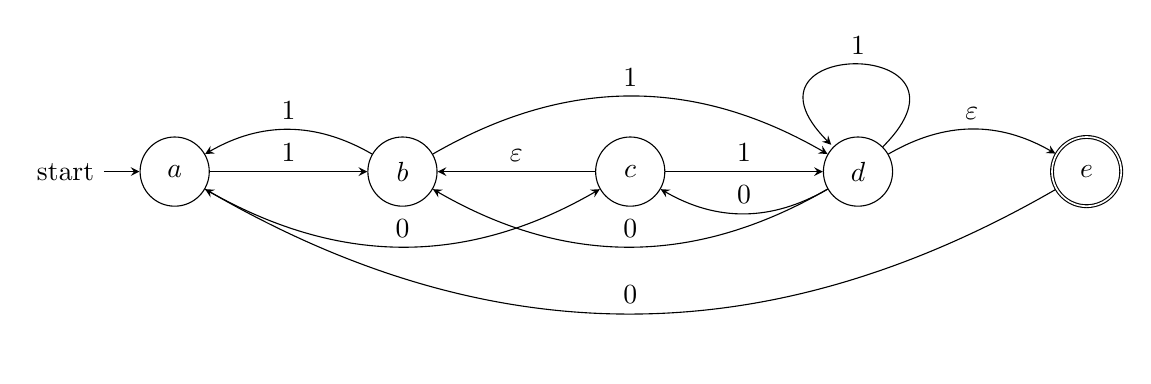
\begin{tikzpicture}[->,>=stealth] 

\node [state,initial] (a){$a$};
\node[state,right = 2cm of a](b){$b$};
\node[state,right = 2cm of b](c){$c$};
\node[state,right = 2cm of c](d){$d$};
\node[state,accepting,right = 2cm of d](e){$e$};


\path (a) edge [above] node{$1$}(b);
\path (a) edge [above,bend right] node{$0$}(c);

\path (b) edge [above,bend left] node{$1$}(d);
\path (b) edge [above,bend right] node{$1$}(a);

\path (c) edge [above] node{$1$}(d);
\path (c) edge [above] node{$\varepsilon$}(b);

\path (d) edge [above,bend left] node{$0$}(c);
\path (d) edge [above,bend left] node{$0$}(b);
\path (d) edge [above,bend left] node{$\varepsilon$}(e);
\path (d) edge [above,loop] node{$1$}(d);

\path (e) edge [above,bend left] node{$0$}(a);
%\path (a) edge [above,bend left] node{$0$}(q1);

%loop

%\path (q0) edge [above,loop] node{$1,2$}(q0);
\end{tikzpicture}

Give the diagram of the non-deterministic finite state machine above, we can find the language that such a machine accepts. Namely \me{L(M) = L. } For the machine above the  regular expression representing the language \me{L} is:\\ \newline

 \me{(0 \cup1)1[(01)^\ast \cup (1 \cup 0)^\ast]^\ast  } \\ \\ \\

(b) a deterministic automaton that is equivalent to N.

\begin{enumerate}
  \item Let  Q' =  $\mathcal{P}(Q)$, where Q = \{a,b,c,d,e\}
  \item The transition map \me{\delta': Q' \times \Sigma \rightarrow Q'} is defined as: \\
  \newpage
 \begin{table}[h!]
\centering
\begin{tabular}{||c c c ||} 
 \hline
 \me{\delta} & 0 & 1  \\ [0.5ex] 
 \hline\hline
 \me{\emptyset} & \me{\emptyset}   &\me{\emptyset}      \\ 
 \me{\{a\}} & \me{\phi}  & \me{\{a,d\}}   \\
 \me{\{b\}}& \me{\{c,b\}}  & \me{\{b\}}       \\
 \me{\{c\}} & \me{\emptyset}  & \me{\{a,d,e\}}   \\
 \me{\{d\}} & \me{\{b,c\}}   & \me{\{d,e\}}          \\ 
 \me{\{e\}} & \me{\{a\}}      & \me{\emptyset}    \\ 
 \me{\{a,b\}} & \me{\{c,e\}}  & \me{\{a,b,d,e\}}   \\
 \me{\{a,c\}} & \me{\{b,c\}}  & \me{\{b,d,e\}}           \\
 \me{\{a,d\}} & \me{\{b,c,e\}}  & \me{\{b,d,e\}}        \\
 \me{\{a,e\}} & \me{\{a,b,c\}}   & \me{\{b\}}          \\ 
 
 
 \me{\{b,c\}} & \me{\emptyset}      & \me{\{a,b,d,e\}}      \\ 
 \me{\{b,d\}} & \me{\{b,c,e\}}  & \me{\{a,d,e\}}   \\
 \me{\{b,e\}} & \me{\{a\}}  & \me{\{a,d,e\}}         \\
 \me{\{c,d\}}& \me{\{b,c,e\}}  & \me{\{d,e\}}       \\
 \me{\{c,e\}} & \me{\{a,b\}}   & \me{\{d,e\}}          \\
 \me{\{d,e\}} & \me{\{a,b,c\}}  & \me{\{d,e\}}        \\
 \me{\{a,b,c\}}& \me{\{b,c\}}      & \me{\{a,b,d,e\}}     \\ 
 \me{\{a,b,d\}} & \me{\{b,c\}}  & \me{\{a,b,d,e\}}   \\
 \me{\{a,b,e\}} & \me{\{a,b,c\}}  & \me{\{a,b,d,e\}}          \\
  \me{\{a,c,d\}} & \me{\{b,c,e\}}  & \me{\{d,e\}}       \\
   \me{\{a,c,e\}}& \me{\{a,b,c\}}   & \me{\{b,d,e\}}         \\
   \me{\{a,d,e\}} & \me{\{a,b,c\}}  & \me{\{b,d,e\}}  \\
  \me{\{b,c,d\}} & \me{\{b,c,e\}}  & \me{\{b,d,e\}}      \\
 \me{\{b,c,e\}}& \me{\{a\}}   & \me{\{a,d,e\}}       \\
  \me{\{b,d,e\}}& \me{\{a,b,c,e\}}   & \me{\{a,d,e\}}    \\

 \me{\{c,d,e\}}& \me{\{a,b,c,\}}      & \me{\{b,d,e\}}   \\ 
 \me{\{a,b,c,d\}}& \me{\{a,b,c,e\}}  & \me{\{a,b,d,e\}}   \\
 \me{\{a,b,c,e\}} & \me{\{a,b,c\}}  & \me{\{a,b,c,d,e\}}      \\
   \me{\{a,b,d,e\}} & \me{\{a,b,c,e\}}  & \me{\{a,b,d,e\}}    \\
     \me{\{a,c,d,e\}}& \me{\{a,b,c\}}   & \me{\{a,b,d,e\}}      \\
  \me{\{b,c,d,e\}} & \me{\{a,b,c\}}      & \me{\{a,d,e\}}    \\ 
   \me{\{a,b,c,d,e\}} & \me{\{a,b,c,e\}}  & \me{\{a,b,d,e\}}     \\[1ex] 
 \hline
\end{tabular}
\caption{}
\label{table:2}
\end{table}

  \item \me{a' = \{a\}}
  \item \me{F=\{\{e\},\{a,e\},\{b,e\},\{c,e\},\{d,e\},\{a,b,e\},\{b,c,e\},\{c,d,e\},\{a,b,c,e\},\{b,c,d,e\},\{a,b,c,d,e\}\}}
  
\end{enumerate}
 %%%%%%%%%%%%%%%%%%% First Question%%%%%%%%%%%%%%%%%%%%%%%%
 
 
 
 %%%%%%%%%%%%%%%%%%% Second Question%%%%%%%%%%%%%%%%%%%%%%%
 \newpage
\paragraph{\Large{Question 2\\ \\}}
Find a proof of the pumping lemma for regular languages based exclusively on regular expressions \textbf{do not use automata}. The first sentence in your proof should be: \textit{Since L is regular, there is a regular expression R representing L}. \\ \\
Proof:

The pumping lemma states the follwing: \\
If \me{L} is a regular language, then there is a number \me{p} such that if \me{r} is any string of \me{L} and has length of at least \me{p}, then  \me{R=xyx} and \me{R} is said to satisfy the following conditions:
\begin{enumerate}
  \item for each \me{i \geq 0, xy^i z \in L} 
  \item \me{|y| > 0}
  \item \me{|xy| \leq p}
\end{enumerate}


Since \me{L} is regular, there is a regular expression \me{R} representing \me{L}. We first consider the case, where \me{R} is not of the length of at least \me{p}. In this case, the pumping lemma would be trivial(true), since the regular expression representing \me{L} meets all of the three conditions. 
\\ \\
 The more interesting case would be when \me{R} is of the length of at least \me{p.} Our assumption is that \me{R} is a regular expression and it can be expressed as \me{R = xyz}. We define \me{p} as the number of nodes of the parsed regular expression in conjunctive normal form of the expression. Since R is a regular expression, we can use the operations defined for regular expressions and ensure the pumping lemma can be met using these operations. Let \me{R = r_1r_2...r_n}, such that \me{|R| = n} and \me{n \geq p}.if we were to expand the parse tree for the string we see there are\me{n+1} concatenation operations or union operations in conjunctive normal (the +1 is due to the root of the tree). Given the above, it means there is at least \me{p+1} operations for the parsing of the regular expression, this is done so to satisfy the bound condition. Among the first \me{p+1} operations, there will be one operation, or node in the parsing  tree, that will contain the same symbol, this is due to the pigeon hole principle. Let us call the first instance of this node in the parsing tree \me{r_j} and the  second \me{r_l.} Given that \me{r_l} node occurs among the nodes closest to the leafs nodes, we have \me{l \leq p+1}. \\
 
 Now we let \me{R =xyz}, such that \me{x=s_1...s_{j-1}} , \me{y=s_j...s_{l-1}} and \me{z=s_l ...s_n.} This is done so\me{ x} takes the part of \me{r_1} to \me{r_j} nodes of the parsing tree, \me{y} takes \me{r_j} \me{r_{l-1}}and \me{z} belongs to \me{r_{j+1}} to \me{r_{n+1}}  of the parsing tree of the regular expression. The regular expression defines \me{R=xy^iz} has the same parsing for \me{i \geq 0}. Condition 1 is met. We know \me{j \neq l}, among the first \me{p+1} nodes in the parsing must contain the same node symbol, so \me{|y| > 0}. Condition 2 is met. We also know that \me{l \leq p+1}, so \me{|xy| \leq p}. Thus we have satisfied all conditions of the pumping lemma.  \\ \\
 
 We have proved that if a language is regular, thus having a regular expression representing such a language, it must therefore satisfy the pumping lemma. 
\ \ \\

	


 %%%%%%%%%%%%%%%%%%% Second Question%%%%%%%%%%%%%%%%%%%%%%%

\end{document}